\documentclass[10pt,a4paper]{article}
\usepackage[utf8]{inputenc}
\usepackage[english]{babel}
\usepackage{csquotes}
\usepackage{amsmath}
\usepackage{amsfonts}
\usepackage{amssymb}
\usepackage{graphicx}
\usepackage[margin=0.5in]{geometry}
\usepackage{amsthm}
\usepackage{enumitem}
\usepackage{tikz}
\usetikzlibrary{calc}
\newtheorem{question}{Question}
\newtheorem*{question*}{Question}
\newtheorem{theorem}{Theorem}
\newtheorem*{theorem*}{Theorem}
\newtheorem{lemma}{Lemma}

\theoremstyle{definition}
\newtheorem{answer}{Answer}
\newtheorem*{answer*}{Answer}


\title{Advanced Calc. Homework 10}
\author{Colin Williams}

\begin{document}
\maketitle

\section*{18.5}
\begin{enumerate}[label = (\alph*)]
\item Let $f$ and $g$ be continuous functions on $[a,b]$ such that $f(a) \geq g(a)$ and $f(b) \leq g(b)$. Prove that $f(x_0) = g(x_0)$ for at least one $x_0 \in [a,b]$.
\item Show Example 1 can be viewed as a special case of part (a).
\end{enumerate}

\begin{proof}{\textbf{(a)}}
\\If $f(a) = g(a)$ or $f(b) = g(b)$, then the result follows immediately, so assume $f(a) \neq g(a)$ and $f(b) \neq g(b)$. Let $h(x) = f(x) - g(x)$, then by Theorem 17.3/Theorem 17.4(i) $h$ is also a continuous function. We can see that $h(a) = f(a) - g(a) > 0$ and $h(b) = f(b) - g(b) < 0$. Additionally $a < b$ by the definition of the interval $[a,b]$. Therefore, by the Intermediate Value Theorem, there exists some $x_0 \in (a,b)$ such that $h(x_0) = 0$. Combining this with the fact that we could possibly have $f(a) = g(a)$ or $f(b) = g(b)$, then we get that $f(x_0) = g(x_0)$ for some $x_0 \in [a,b]$.
\end{proof}

\begin{answer*}{\textbf{(b)}}
\\In Example 1, we showed that for a continuous function $f: [0,1] \to [0,1]$, then $f(x_0) = x_0$ for some $x_0 \in [0,1]$. This is equivalent to part (a) of this question for $[a,b] = [0,1]$ and $g(x) = x$ since $f(a) = f(0) \geq g(0) = 0$ and $f(b) = f(1) \leq g(1) = 1$ due to $f$ being contained in $[0,1]$.
\end{answer*}

\section*{18.6}
Prove $x = \cos(x)$ for some $x \in \left(0, \frac{\pi}{2}\right)$.

\begin{proof}{$ $}
\\Note that if we let $f(x) = \cos(x)$ and $g(x) = x$, then we can see that $f(0) = 1 \geq 0 = g(0)$ and $f\left(\frac{\pi}{2}\right) = 0 \leq \frac{\pi}{2} = g\left(\frac{\pi}{2}\right)$. Thus, from Exercise 18.5(a) (and the fact that $f$ and $g$ are both continuous), we can conclude that there exists some $x_0 \in \left[0, \frac{\pi}{2}\right]$ such that $f(x_0) = g(x_0)$. However, we have just seen that $f(0) \neq g(0)$ and $f\left(\frac{\pi}{2}\right) \neq g\left(\frac{\pi}{2}\right)$, so that means there does indeed exist some $x \in \left(0, \frac{\pi}{2}\right)$ such that $x = \cos(x)$.
\end{proof}

\section*{18.7}
Prove $xe^x = 2$ for some $x$ in $(0,1)$.

\begin{proof}{$ $}
\\Let $f(x) = xe^x$, then $f$ is a continuous function by the continuity of $e^x$ and $x$ and Theorem 17.4(ii). Furthermore, note that $f(0) = 0e^0 = 0 < 2$ and $f(1) = 1e^1 \approx 2.718 > 2$. Thus, by the Intermediate Value Theorem, there exists some $x_0 \in (0,1)$ such that $f(x_0) = 2$, proving the statement. 
\end{proof}

\section*{18.8}
Suppose $f$ is a real-valued continuous function on $\mathbb{R}$ and $f(a)f(b) < 0$ for some $a,b \in \mathbb{R}$. Prove there exists $x$ between $a$ and $b$ such that $f(x) = 0$.

\begin{proof}{$ $}
\\Let $I$ be defined as follows:
\[I := 
\begin{cases}
[a,b] &\text{if $a<b$}\\
[b,a] &\text{if $b<a$}
\end{cases}\]
Furthermore, without loss of generality, assume that $f(a) > f(b)$ (if not, we can simply reverse the roles of $a$ and $b$ and note that $I$ is defined appropriately to allow this. Also see that we cannot have $f(a) = f(b)$ as this would cause $f(a)f(b) = f(a)^2 \geq 0$). It is clear that $f(a) \neq 0$ and $f(b) \neq 0$ since the opposite of this would cause $f(a)f(b) = 0$ which is not true. Therefore, since $f(a)f(b) < 0$, we must have that the sign of $f(a)$ differs from the sign of $f(b)$ because if they were the same, then $f(a)f(b) > 0$ which is not true. Thus, since $f(a) > f(b)$ and they have different signs, we can conclude that $f(a) > 0$ and $f(b) < 0$. Then, by the continuity of $f$, we can apply the Intermediate Value Theorem to conclude that there exists some $x \in I$ such that $f(x) = 0$.
\end{proof}

\section*{18.9}
Prove that a polynomial function $f$ of odd degree has at least one real root.

\begin{proof}{$ $}
\\Let $f(x) = a_nx^n + a_{n - 1}x^{n-1} + \cdots + a_1x + a_0$ be an arbitrary polynomial with $n \in \mathbb{N}$ odd. Without loss of generality, assume that $a_n = 1$ (if not, simply consider the rest of this proof with the function $\left(\frac{1}{a_n}\right)f$). Thus, we are considering $f(x) = x^n + a_{n - 1}x^{n-1} + \cdots + a_1x + a_0$. This is equivalent to 
\begin{equation}
f(x) = x^n\left(1 + \frac{a_{n - 1}x^{n - 1} + \cdots + a_1x + a_0}{x^n}\right)
\end{equation}
Taking limits as $x$ goes to $\pm \infty$ leaves the bracketed term irrelevant since 
\begin{align*}
\lim_{x \to \pm \infty} 1 + \frac{a_{n - 1}x^{n - 1} + \cdots + a_1x + a_0}{x^n} &= \lim_{x \to \pm \infty} 1 + \frac{a_{n-1}}{x} + \cdots + \frac{a_1}{x^{n-1}} + \frac{a_0}{x^n}\\
&= 1 + 0 + \cdots + 0 + 0\\
&= 1.
\end{align*}
Thus, $\displaystyle \lim_{x \to \infty}f(x) = \lim_{x \to \infty} x^n = +\infty$ and $\displaystyle \lim_{x \to -\infty}f(x) = \lim_{x \to -\infty}x^n = -\infty$ since $n$ is odd and any negative number to an odd power is negative (since $p^{2k + 1} = p^{2k}\cdot p = c\cdot p < 0$ for $c$ some positive number). In particular, this means that there exists some $a < 0$ such that $f(a) < 0$ and there exists some $b > 0$ such that $f(b) > 0$ which means we can use the Intermediate Value Theorem to indicate that there exists some $x_0 \in (a,b)$ such that $f(x_0) = 0$, making $x_0$ a root for $f$.
\end{proof}

\section*{18.10}
Suppose $f$ is continuous on $[0,2]$ and $f(0) = f(2)$. Prove there exist $x,y \in [0,2]$ such that $|y - x| = 1$ and $f(x) = f(y)$. 

\begin{proof}{$ $}
\\Consider $g(x) = f(x + 1) - f(x)$ on $[0,1]$. From this, we have that $g(0) = f(1) - f(0)$ and $g(1) = f(2) - f(1) = f(0) - f(1) = -g(0)$. The important relationship here is that $g(1) = -g(0)$. If $g(0) = 0$, then clearly we have $f(1) = f(0)$ or if $g(1) = 0$, then we have that $f(2) = f(1)$ which both satisfy the condition we which to show. Otherwise, $g(0)$ and $g(1)$ have different signs. Thus the point $0$ lies in between $g(0)$ and $g(1)$ which indicates (along with the possibility that $g(0) = 0$ or $g(1) = 0$) that there exists some $x_0 \in [0,1]$ such that $g(x_0) = 0 \iff f(x_0 + 1) = f(x_0)$ which clearly satisfies the statement we are trying to prove with $x = x_0$ and $y = x_0 + 1$.
\end{proof}

\section*{19.1}
Which of the following continuous functions are uniformly continuous on the specified set? Justify your answers by using any theorems.
\begin{enumerate}[label = (\alph*)]
\item $f(x) = x^{17}\sin(x) - e^x\cos(3x)$ on $[0, \pi]$,
	\begin{itemize}
	\item This is \boxed{\text{uniformly continuous}} since we know that $x^{17}, \sin(x), e^x,$ and $\cos(3x)$ are all continuous functions (thus, their sum and product is continuous). Therefore, since $f$ is continuous on a closed interval, $[0, \pi]$, Theorem 19.2 assures us that $f$ is uniformly continuous on $[0,\pi]$.
	\end{itemize}
\item $f(x) = x^3$ on $[0,1]$,
	\begin{itemize}
	\item This is \boxed{\text{uniformly continuous}} since we know that $x^3$ is continuous. Thus, $f$ is continuous on $[0,1]$, so Theorem 19.2 assures us that $f$ is uniformly continuous on $[0,1]$.
	\end{itemize}
\item $f(x) = x^3$ on $(0,1)$,
\begin{itemize}
	\item If we make the extension
	\[\tilde{f}(x) = \begin{cases}
	f(x) &\text{for } x\in (0,1)\\
	0 &\text{for } x = 0\\
	1 &\text{for } x = 1
	\end{cases}\]
	Then $\tilde{f}$ is continuous on $[0,1]$ since for any sequence $(s_n) \subset (0,1)$ converging to 0, we have $\tilde{f}(s_n) = f(s_n) = s_n^3$ which converges to $\tilde{f}(0) = 0$ and for any sequence $(t_n) \subset (0,1)$ converging to 1, we have $\tilde{f}(t_n) = f(t_n) = t_n^3$ which converges to $\tilde{f}(1) = 1$ and clearly $\tilde{f}$ is continuous in $(0,1)$ by the continuity of $x^3$. Thus, $\tilde{f}$ is continuous on $[0,1]$, so it must be uniformly continuous on $[0,1]$ by Theorem 19.2. Furthermore, this means that $f$ must be \boxed{\text{uniformly continuous}} on $(0,1)$.
	\end{itemize}
\item $f(x) = x^3$ on $\mathbb{R}$,
	\begin{itemize}
	\item Assume that $f$ is uniformly continuous on $\mathbb{R}$. Then by Definition 19.1, we know that that there exists some $\delta > 0$ such that $x, y \in \mathbb{R}$ and $|x - y| < \delta$ implies that $|x^3 - y^3| < 1$. In this case, choose $y = x + \frac{\delta}{2}$ which gives the following:
	\begin{align*}
	|x_3 - y^3| = |x - y||x^2 + xy + y^2| &= \left|x - \left(x + \frac{\delta}{2}\right)\right|\left|x^2 + x\left(x + \frac{\delta}{2}\right) + \left(x + \frac{\delta}{2}\right)^2\right|\\
	&= \frac{\delta}{2}\left|3x^2 + \frac{3\delta}{2}x + \frac{\delta}{4}\right|\\
	&> \frac{\delta}{2}\left|\frac{2}{\delta} + \frac{3\delta}{2}\sqrt{\frac{2}{3\delta}} + \frac{\delta}{4}\right| &\text{whenever $x > \sqrt{\frac{2}{3\delta}}$}\\
	&> \frac{\delta}{2}\left|\frac{2}{\delta}\right| &\text{since $\frac{3\delta}{2}\sqrt{\frac{2}{3\delta}} + \frac{\delta}{4} > 0$}\\
	&= 1
	\end{align*}
	Thus, we have shown that for $y = x + \frac{\delta}{2}$ and $x > \sqrt{\frac{2}{3\delta}}$ that $|f(x) - f(y)| > 1$ which means that $f$ is \boxed{\text{not uniformly continuous}}.
	\end{itemize}
\item $f(x) = \frac{1}{x^3}$ on $(0,1]$,
	\begin{itemize}
	\item Theorem 19.4 tells us that if $f$ is uniformly continuous on a set $S$ and $(s_n)$ is a Cauchy sequence in $S$, then $(f(s_n))$ is a Cauchy sequence. However, taking $(s_n) = \frac{1}{n}$ gives us $s_n \in (0,1]$ for all $n$ and $(s_n)$ is a Cauchy sequence. However, $f(s_n) = \frac{1}{(1/n)^3} = n^3$ which is not a Cauchy sequence since it is not convergent; thus, $f$ is \boxed{\text{not uniformly continuous}}.
	\end{itemize}
\item $f(x)= \sin\left(\frac{1}{x^2}\right)$ on $(0,1]$,
	\begin{itemize}
	\item Let's once again use Theorem 19.4. In this case, take $(s_n) = \sqrt{\frac{2}{\pi + 2n\pi}}$. It is easy to see that $s_n \in (0,1]$ for all $n$ and it is easy to see that $(s_n)$ is Cauchy since it is a convergent sequence. However, $f(s_n) = \sin\left(\frac{1}{\sqrt{\frac{2}{\pi + 2n\pi}}^2}\right) = \sin\left(\frac{\pi}{2} + n\pi\right)$. We can see that $f(s_n)$ is not Cauchy since the subsequence with odd indices converges to $-1$ and the subsequence with even indices convergest o $1$. Thus, $f(s_n)$ is not convergent, so it is not Cauchy which implies that $f$ is \boxed{\text{not uniformly convergent}}.
	\end{itemize}
\item $f(x) = x^2\sin\left(\frac{1}{x}\right)$ on $(0,1]$.
	\begin{itemize}
	\item Let's make the following extension of $f$:
	\[\tilde{f}(x) = \begin{cases}
	f(x) &\text{for } x \in (0,1]\\
	0 &\text{for } x = 0
	\end{cases} \]
	I will first show that $\tilde{f}$ is continuous in its domain, $[0,1]$. Note for all $x \in (0,1]$, $\tilde{f}$ is clearly continuous since $x^2$, $\sin(x)$, and $\frac{1}{x}$ are all continuous when $x \neq 0$. Thus, the only point of contention is $x = 0$, so I will examine the continuity of $\tilde{f}$ at $x = 0$. Let $\varepsilon > 0$ be fixed and consider $|\tilde{f}(x) - \tilde{f}(0)| = |\tilde{f}(x)| = \left|x^2\sin\left(\frac{1}{x}\right)\right| \leq |x^2|$. Thus choosing $\delta = \sqrt{\varepsilon}$ we get $|x - 0| = |x| < \sqrt{\varepsilon}$ which implies that $|\tilde{f}(x) - \tilde{f}(0)| \leq |x^2| < \left|\sqrt{\varepsilon}^2\right| = \varepsilon$. Thus, $\tilde{f}$ is continuous at $x = 0$, so $\tilde{f}$ is continuous in all of $[0,1]$, so Theorem 19.2 tells us that $\tilde{f}$ is uniformly continuous on $[0,1]$ which further means that $f$ is \boxed{\text{uniformly continuous}} on $(0,1]$.
	\end{itemize}
\end{enumerate}

\section*{19.2}
Prove each of the following functions is uniformly continuous on the indicated set by directly verifying the $\varepsilon$--$\delta$ property in Definition 19.1.
\begin{enumerate}[label = (\alph*)]
\item $f(x) = 3x + 11$ on $\mathbb{R}$, 
	\begin{itemize}
	\item Let $\varepsilon > 0$ be fixed and let $x,y \in \mathbb{R}$. Let's first consider the following:
	\begin{align*}
	|f(x) - f(y)| = |3x + 11 - (3y + 11)| = 3|x - y|
	\end{align*}
	Thus, choosing $\delta = \frac{\varepsilon}{3}$ gives us $|x - y| < \frac{\varepsilon}{3}$. Therefore, we have $|f(x) - f(y)| = 3|x - y| < 3 \cdot \frac{\varepsilon}{3} = \varepsilon$ satisfying the definition of uniform continuity.
	\end{itemize}
\item $f(x) = x^2$ on $[0,3]$,
	\begin{itemize}
	\item Let $\varepsilon > 0$ be fixed and let $x,y \in [0,3]$. Let's first consider the following:
	\begin{align*}
	|f(x) - f(y)| = |x^2 - y^2| = |x - y||x + y|
	\end{align*}
	Note that since $x,y \in [0,3]$, $|x + y| \leq 6$ for any $x,y$. Thus, choosing $\delta = \frac{\varepsilon}{6}$ gives $|x - y| < \frac{\varepsilon}{6}$ which in turn leads to $|f(x) - f(y)| = |x - y||x + y| \leq |x - y| \cdot 6 < \frac{\varepsilon}{6} \cdot 6 = \varepsilon$, satisfying the definition of uniform continuity.
	\end{itemize}
\item $f(x) = \frac{1}{x}$ on $\left[\frac{1}{2}, \infty\right)$.
	\begin{itemize}
	\item Let $\varepsilon > 0$ be fixed and let $x,y \in \left[\frac{1}{2}, \infty\right)$. Let's first consider the following:
	\begin{align*}
	|f(x) - f(y)| = \left|\frac{1}{x} - \frac{1}{y}\right| = \left|\frac{y - x}{xy}\right| = \frac{|x - y|}{|xy|}
	\end{align*}
	Note that since $x,y \geq \frac{1}{2}$, $|xy| \geq \frac{1}{4} \implies \frac{1}{|xy|} \leq 4$. With this in mind, choose $\delta = \frac{\varepsilon}{4}$ which gives $|x - y| < \frac{\varepsilon}{4}$. Using this with the estimate above we get $|f(x) - f(y)| = \frac{|x -y|}{|xy|} \leq 4|x - y| < 4 \cdot \frac{\varepsilon}{4} = \varepsilon$, satisfying the definition of uniform continuity.
	\end{itemize}
\end{enumerate}

\section*{19.5}
Which of the following continuous functions is uniformly continuous on the specified set? Justify your answers, using appropriate theorems.
\begin{enumerate}[label = (\alph*)]
\item $\tan(x)$ on $\left[0, \frac{\pi}{4}\right]$,
	\begin{itemize}
	\item Since $\tan(x) = \frac{\sin(x)}{\cos(x)}$ and $\sin(x)$ and $\cos(x)$ are both continuous in $\left[0, \frac{\pi}{4}\right]$ and $\cos(x) \neq 0$ for any $x \in \left[0, \frac{\pi}{4}\right]$, then we can apply Theorem 17.4(iii) to conclude that $\tan(x)$ is continuous on $\left[0, \frac{\pi}{4}\right]$. From this, we can use Theorem 19.2 to conclude that $\tan(x)$ is \boxed{\text{uniformly continuous}} on $\left[0, \frac{\pi}{4}\right]$.
	\end{itemize}
\item $\tan(x)$ on $\left[0, \frac{\pi}{2}\right)$,
	\begin{itemize}
	\item According to Exercise 19.4(a), if a function is uniformly continuous on a bounded set $S$, then that function is also bounded on $S$. In our case here $S = \left[0, \frac{\pi}{2}\right)$ is our bounded set. However, $\lim_{x \to \frac{\pi}{2}^-}\tan(x) = +\infty$, which indicates that $\tan(x)$ is not bounded on $S$, thus $\tan(x)$ is \boxed{\text{not uniformly continuous}}.
	\end{itemize}
\item $\frac{1}{x}\sin^2(x)$ on $(0, \pi]$,
	\begin{itemize}
	\item In Example 9 on Page 149, they defined 
	\[\tilde{h}(x) = \begin{cases}
	\frac{\sin(x)}{x} &\text{for } x \neq 0\\
	1 &\text{for } x = 0
	\end{cases}\]
	where the domain of $\tilde{h}$ was $\mathbb{R}$. They find that that $\tilde{h}$ is uniformly continuous on this domain. If instead, we restrict the domain to $[0,\pi]$ then it would still be a uniformly continuous function. Thus, define the following function:
	\[f(x) = \begin{cases}
	\frac{\sin^2(x)}{x} &\text{for } x \in (0,\pi]\\
	0 &\text{for } x = 0
	\end{cases}
	\]
	It is clear that $f(x) = \sin(x)\tilde{h}(x)$ for $\tilde{h}$ restricted to the domain $[0,\pi]$. Thus, by the continuity of $\sin(x)$ and the Example 9 determining that $\tilde{h}$ was also continuous, we can conclude that $f$ is continuous on $[0,\pi]$. Using Theorem 19.5 therefore tells us that $\frac{\sin^2(x)}{x}$ on $(0, \pi]$ is a \boxed{\text{uniformly continuous}} function. 
	\end{itemize}
\item $\frac{1}{x - 3}$ on $(0,3)$,
	\begin{itemize}
	\item Using exercise 19.4(a), we can note that this function is not bounded on $(0,3)$, specifically as $x$ approaches 3, so it must be \boxed{\text{not uniformly continuous}}.
	\end{itemize}
\item $\frac{1}{x - 3}$ on $(3,\infty)$,
	\begin{itemize}
	\item Using the same reasoning we did for part (d) of this question, we can note that this function is not bounded on $(3, \infty)$, once again where $x$ approaches 3, so Exercise 19.4(a) tells us that this function must be \\\boxed{\text{not uniformly continuous}}
	\end{itemize}
\item $\frac{1}{x - 3}$ on $(4,\infty)$.
	\begin{itemize}
	\item Recall the derivative of $\frac{1}{x - 3}$ is $\frac{-1}{(x - 3)^2}$. Furthermore, note that this derivative is bounded on $(4, \infty)$ since $\left|\frac{-1}{(x - 3)^2}\right| < 1$ for all $x > 4$. Thus, by using Theorem 19.6, we can say that this function is \boxed{\text{uniformly continuous}}.
	\end{itemize}
\end{enumerate}

\section*{19.6}
\begin{enumerate}[label = (\alph*)]
\item Let $f(x) = \sqrt{x}$ for $x \geq 0$. Show $f'$ is unbounded on $(0,1]$ but $f$ is nevertheless uniformly continuous on $(0,1]$. Compare with Theorem 19.6.
	\begin{itemize}
	\item By using the power rule, $f'(x) = \frac{1}{2\sqrt{x}}$. This is unbounded on $(0,1]$ because for any $M > 0$, we can find a $\delta > 0$ such that $|x| < \delta$ implies that $|f'(x)| > M$. Let $\delta = \frac{1}{4M^2}$. This yields, $|f'(x)| = \left|\frac{1}{2\sqrt{x}}\right| > \left|\frac{1}{2\sqrt{1/(4M^2)}}\right| = \left|\frac{2M}{2}\right| = M$, which shows $f'$ is unbounded. Despite this, $f$ is still uniformly continuous on $(0,1]$. We can show this by noting that $\sqrt{x}$ is continuous on $[0,1]$ thus, by Theorem 19.2, $\sqrt{x}$ is uniformly continuous on $[0,1]$ and by Theorem 19.5 this shows that $f$ is uniformly continuous on $(0,1]$. This shows that the converse to Theorem 19.6 is not true -- just because a function has an unbounded derivative does not mean it must be not uniformly continuous. 
	\end{itemize}
\item Show $f$ is uniformly continuous on $[1,\infty)$.
	\begin{itemize}
	\item Let $\varepsilon > 0$ be fixed and let $x,y \in [1,\infty)$, then let's examine the following:
	\begin{align*}
	|f(x) - f(y)| = |\sqrt{x} - \sqrt{y}| = \left|\frac{x - y}{\sqrt{x} + \sqrt{y}}\right| = \frac{|x -y|}{\sqrt{x} + \sqrt{y}}
	\end{align*}
	Note that $\sqrt{x} + \sqrt{y} \geq 2$ for all $x,y \geq 1$ which means that $\frac{1}{\sqrt{x} + \sqrt{y}} \leq \frac{1}{2}$ for all $x, y \geq 1$. This motivates the choice of $\delta = 2\varepsilon$, i.e. $|x - y| < 2\varepsilon$. From this, we get $|f(x) - f(y)| = \frac{|x - y|}{\sqrt{x} + \sqrt{y}} \leq \frac{1}{2}|x - y| < \frac{1}{2}(2\varepsilon) = \varepsilon$, proving that $f$ is uniformly continuous on $[1,\infty)$.
	\end{itemize}
\end{enumerate}

\section*{20.1}
Sketch the function $\displaystyle f(x) = \frac{x}{|x|}$. Determine, by inspection, the limits: $\displaystyle \lim_{x \to \infty} f(x), \lim_{x \to 0^+} f(x), \lim_{x \to 0^-} f(x), \lim_{x \to -\infty} f(x)$, and $\displaystyle \lim_{x \to 0} f(x)$ if they exist, or indicate when they do not exist.

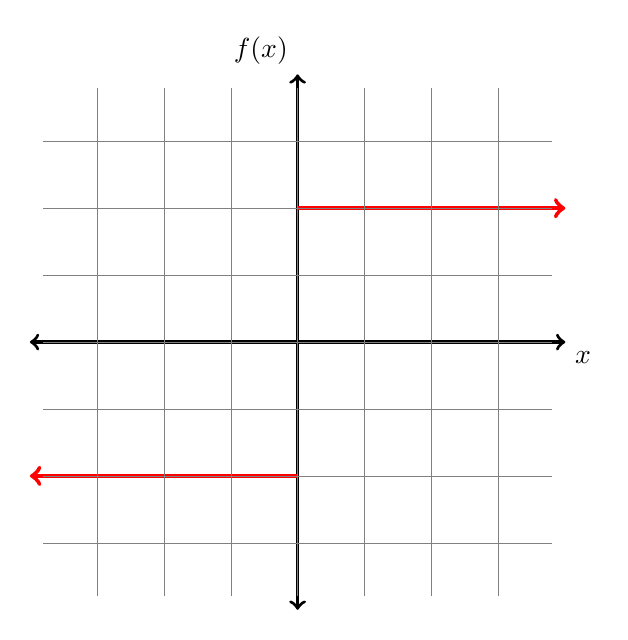
\begin{tikzpicture}[scale = 1.7]
\draw [very thick, <->] (-2,0) -- (2,0);
\node [below right] at (2,0) {$x$};
\draw [very thick, <->] (0,-2) -- (0,2);
\node [above left] at (0,2) {$f(x)$};
\draw [red, ultra thick, ->] (0,1) -- (2,1);
\draw [red, ultra thick, ->] (0,-1) -- (-2, -1);
\draw[step=0.5,gray, ultra thin] (-1.9,-1.9) grid (1.9,1.9);
\end{tikzpicture}

From this picture, we can conclude the following:
\begin{itemize}
\item $\displaystyle \lim_{x \to \infty}f(x) = 1$
\item $\displaystyle \lim_{x \to 0^+}f(x) = 1$
\item $\displaystyle \lim_{x \to 0^-}f(x) = -1$
\item $\displaystyle \lim_{x \to -\infty}f(x) = -1$
\item $\displaystyle \lim_{x \to 0}f(x)$ does not exist.
\end{itemize}

\section*{20.2}
Sketch the function $\displaystyle f(x) = \frac{x^3}{|x|}$. Determine, by inspection, the limits: $\displaystyle \lim_{x \to \infty} f(x), \lim_{x \to 0^+} f(x), \lim_{x \to 0^-} f(x), \lim_{x \to -\infty} f(x)$, and $\displaystyle \lim_{x \to 0} f(x)$ if they exist, or indicate when they do not exist.

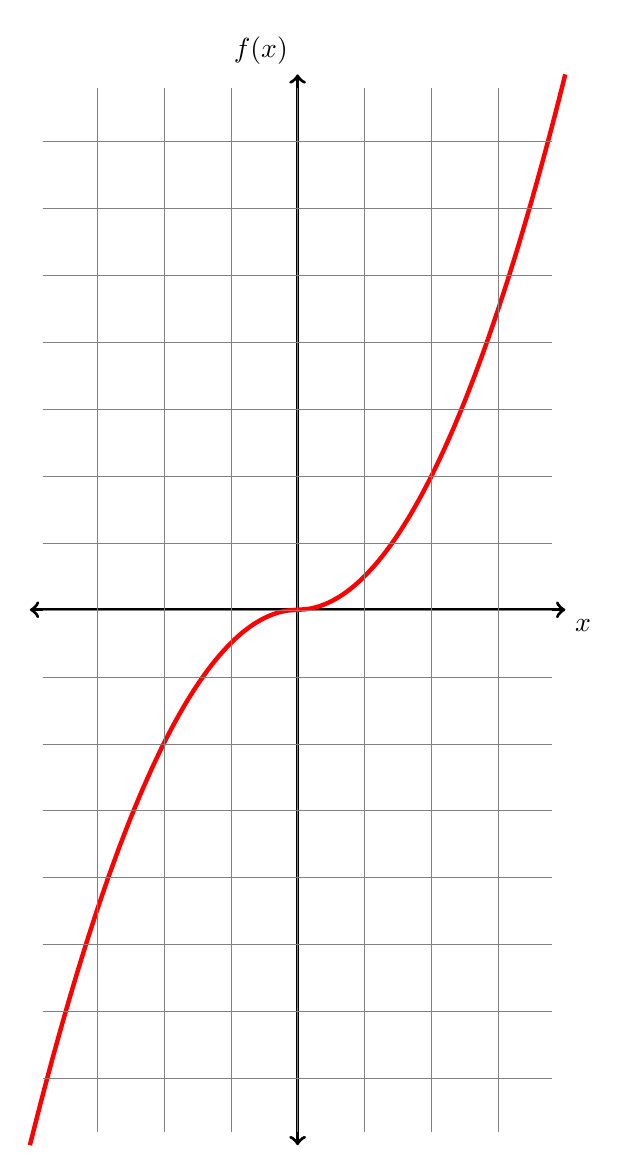
\begin{tikzpicture}[scale = 1.7]
\draw [very thick, <->] (-2,0) -- (2,0);
\node [below right] at (2,0) {$x$};
\draw [very thick, <->] (0,-4) -- (0,4);
\node [above left] at (0,4) {$f(x)$};
\draw [domain=0:2,smooth,variable=\x,red, ultra thick] plot ({\x}, 
 {\x^2});
\draw [domain=-2:0,smooth,variable=\x,red, ultra thick] plot ({\x}, 
 {-1*(\x*\x)});
\draw[step=0.5,gray, ultra thin] (-1.9,-3.9) grid (1.9,3.9);
\end{tikzpicture}

From this picture, we can conclude the following:
\begin{itemize}
\item $\displaystyle \lim_{x \to \infty}f(x) = \infty$
\item $\displaystyle \lim_{x \to 0^+}f(x) = 0$
\item $\displaystyle \lim_{x \to 0^-}f(x) = 0$
\item $\displaystyle \lim_{x \to -\infty}f(x) = -\infty$
\item $\displaystyle \lim_{x \to 0}f(x) = 0$
\end{itemize}

\section*{20.3}
Sketch the function $\displaystyle f(x) = \frac{\sin(x)}{|x|}$. Determine, by inspection, the limits: $\displaystyle \lim_{x \to \infty} f(x), \lim_{x \to 0^+} f(x), \lim_{x \to 0^-} f(x), \lim_{x \to -\infty} f(x)$, and $\displaystyle \lim_{x \to 0} f(x)$ if they exist, or indicate when they do not exist.

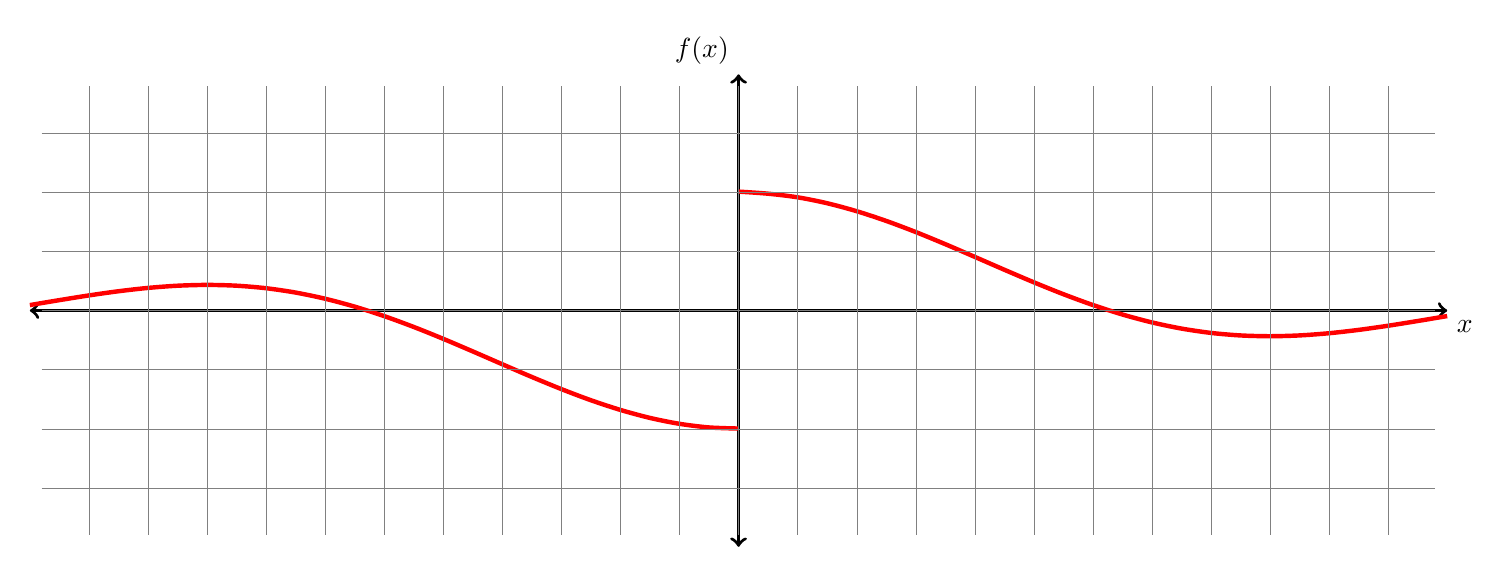
\begin{tikzpicture}[scale = 1.5]
\draw [very thick, <->] (-6,0) -- (6,0);
\node [below right] at (6,0) {$x$};
\draw [very thick, <->] (0,-2) -- (0,2);
\node [above left] at (0,2) {$f(x)$};
\draw [domain=.001:6,smooth,variable=\x,red, ultra thick] plot ({\x}, 
 {sin((180)/(pi) * \x)/\x});
 \draw [domain=-6:-.001,smooth,variable=\x,red, ultra thick] plot ({\x}, 
 {(-1)*sin((180)/(pi) * \x)/\x});
\draw[step=0.5,gray, ultra thin] (-5.9,-1.9) grid (5.9,1.9);
\end{tikzpicture}

From this picture, we can conclude the following:
\begin{itemize}
\item $\displaystyle \lim_{x \to \infty}f(x) = 0$
\item $\displaystyle \lim_{x \to 0^+}f(x) = 1$
\item $\displaystyle \lim_{x \to 0^-}f(x) = -1$
\item $\displaystyle \lim_{x \to -\infty}f(x) = 0$
\item $\displaystyle \lim_{x \to 0}f(x)$ does not exist.
\end{itemize}

\section*{20.4}
Sketch the function $\displaystyle f(x) = x\sin\left(\frac{1}{x}\right)$. Determine, by inspection, the limits: $\displaystyle \lim_{x \to \infty} f(x), \lim_{x \to 0^+} f(x), \lim_{x \to 0^-} f(x), \lim_{x \to -\infty} f(x)$, and $\displaystyle \lim_{x \to 0} f(x)$ if they exist, or indicate when they do not exist.

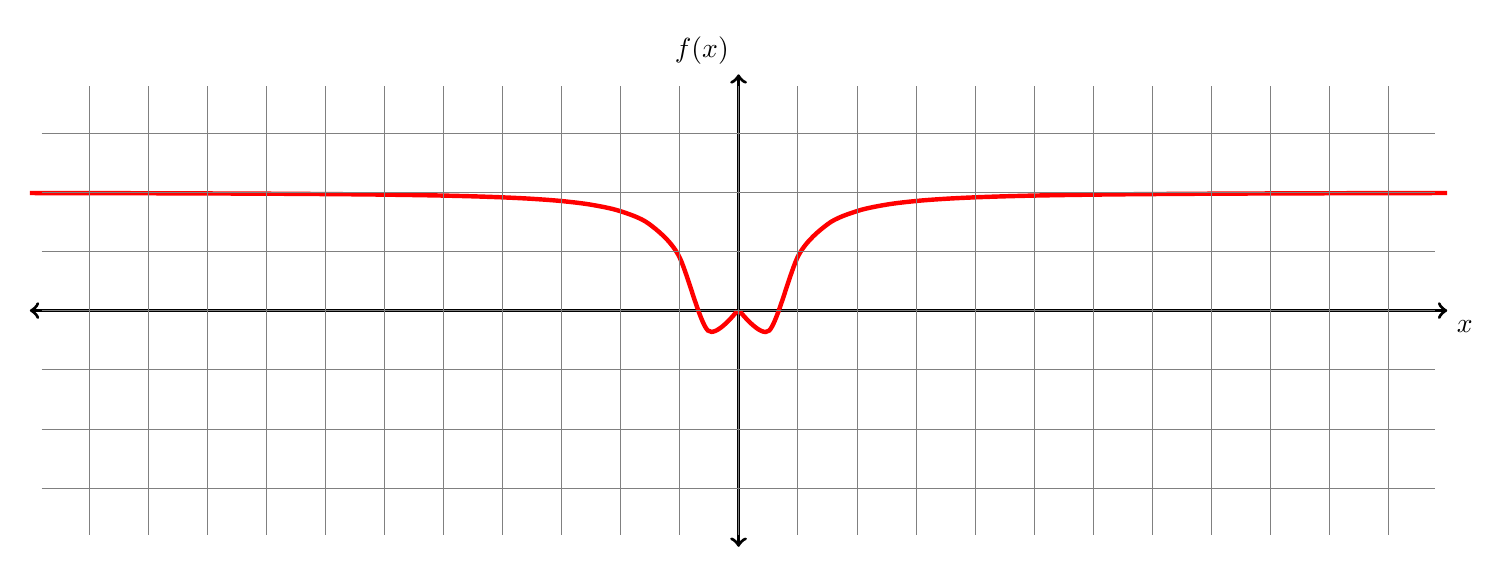
\begin{tikzpicture}[scale = 1.5]
\draw [very thick, <->] (-6,0) -- (6,0);
\node [below right] at (6,0) {$x$};
\draw [very thick, <->] (0,-2) -- (0,2);
\node [above left] at (0,2) {$f(x)$};
\draw [domain=.01:6,smooth,variable=\x,red, ultra thick] plot ({\x}, 
 {\x * sin((180)/(pi) * (1/\x))});
\draw [domain=-6:-.01,smooth,variable=\x,red, ultra thick] plot ({\x}, {\x * sin((180)/(pi) * (1/\x))});
\draw[step=0.5,gray, ultra thin] (-5.9,-1.9) grid (5.9,1.9);
\end{tikzpicture}

From this picture, we can conclude the following:
\begin{itemize}
\item $\displaystyle \lim_{x \to \infty}f(x) = 1$
\item $\displaystyle \lim_{x \to 0^+}f(x) = 0$
\item $\displaystyle \lim_{x \to 0^-}f(x) = 0$
\item $\displaystyle \lim_{x \to -\infty}f(x) = -1$
\item $\displaystyle \lim_{x \to 0}f(x) = 0$
\end{itemize}



\end{document}